\documentclass[7 pt]{article}
\usepackage[toc,page]{appendix}
\usepackage{graphicx}
\usepackage{epstopdf}
\usepackage{caption}
\usepackage{subcaption}
\usepackage{subfig} 
\usepackage{latexsym}
\usepackage{amsmath}
\usepackage{abstract}
\usepackage{amssymb}
\usepackage{amsbsy}
\usepackage{cancel}
\usepackage{multicol}
\usepackage[margin=0.75in]{geometry}

\pagestyle{plain}
\setlength{\columnsep}{2pc}


\title{ {\huge Face and digit classification with CKFD} \\
\begin{center}
\end{center}
{Aristotle University of Thessaloniki} \\
\vspace{10mm}
{\Large Karalias Nikolaos}
}
\date{November 2015}



\begin{document}
\maketitle


\begin{abstract}
In this assignment, we are going to be using the complete Kernel Fisher Discriminant(CKFD) framework introduced by Yang et al. for the purposes of digit and face classification on the databases of MNIST and Olivetti respectively.

\end{abstract}

\bigskip \bigskip
\begin{multicols}{2}
\section{Introduction} \bigskip
Many prevalent algorithms  in statistics and machine learning are most often linear which can be insufficient when dealing with data that has complex non-linear structure. A potential way to alleviate this would be to project the data on to a higher dimensional feature space and execute our linear methods there. Unfortunately, performing this kind of procedure can have a very high computational cost and is therefore impractical in most cases. A potential solution that will allow us to gain some of the benefits of this kind of mapping is the kernel trick. Essentially, it is known from functional analysis that applying a nonlinear kernel(e.g a gaussian) on a dot product in the input space, corresponds to a dot product in a higher dimensional Hilbert space, if a suitable kernel that satisfies certain conditions is selected.\cite{smola06}
 
 This has led to the formulation of many known algorithms in terms of dot products for the purpose of then utilizing the kernel trick; popular algorithms like SVMs and Kernel PCA  which we mentioned earlier. \cite{hof06}
 

The main focus here is going to be the CKFD method developed in  \cite{yang05} and its application
on digit and face recognition. It is a method that combines the principles of Kernel Principal Component Analysis\cite{schol98} and Kernel Fisher Discriminant Analysis\cite{schol99}.

\section{Preliminaries}
We will introduce the main tools that will be required for the CKFD framework.
\subsection{Kernel PCA}
Given a set of observations $\mathbf{x}_k, \; k=1,2,\dots,M, \quad \mathbf{x}_{k} \in \mathbb{R}^{N} $ that are guaranteed to be centered, i.e 
\begin{equation}
\sum_{k=1}^{M} \mathbf{x}_{k}=0,
\end{equation}
PCA projects the data along the axes of maximal variance, diagonalizing the sample covariance matrix which is defined as 
\begin{equation}
\mathbf{C}=\frac{1}{M}\sum_{j=1}^{M}\mathbf{x}_{j}\mathbf{x}_{j}^{\mathbf{T}}.
\end{equation}
This is achieved by solving 
\begin{equation}
\lambda \mathbf{v} = \mathbf{Cv}, \label{eq:covdiag}
\end{equation}
where the eigenvectors $\mathbf{v}$ corresponding to the largest eigenvalues $\lambda$ are the the principal components and directions of maximal variance.

We can write 
\begin{equation}
\mathbf{Cv}=\frac{1}{M}\sum_{j=1}^{M}(\mathbf{x}_{j} \cdot \mathbf{v}) \mathbf{x}_{j}
\end{equation}
and because all solutions of \eqref{eq:covdiag} for $\lambda \geq 0$ must lie in the span of $\mathbf{x}_{k}$, \eqref{eq:covdiag} can be written as 
\begin{equation}
\lambda(\mathbf{x}_{k} \cdot \mathbf{v})= (\mathbf{x}_{k} \cdot \mathbf{Cv}), \quad  k=1,2,\dots,M. \label{eq:modfifdiag}
\end{equation}

For Kernel PCA the same process can be executed but this time in a higher dimensional feature space $\mathcal{H}$ which is related to the input space by the mapping 
\begin{equation}
\Phi : \mathbb{R}^{N} \rightarrow \mathcal{H}, \quad {x}\rightarrow \Phi({x}).
\end{equation}
Equivalently the sample covariance matrix on the feature space is defined as 
\begin{equation}
\mathbf{\tilde{C}}=\frac{1}{M}\sum_{j=1}^{M}\Phi(\mathbf{x}_{j})\Phi(\mathbf{x}_{j})^{\mathbf{T}}.
\end{equation}
Then \eqref{eq:modfifdiag} in the feature space corresponds to
\begin{equation}
\lambda(\Phi(\mathbf{x}_{k}) \cdot \mathbf{u})= (\Phi(\mathbf{x}_{k}) \cdot \mathbf{\tilde{C}u}), \quad  k=1,2,\dots,M. \label{eq:modfifdiagfeat}
\end{equation}
where $\mathbf{u}$ are the eigenvectors in the feature space.
Finally it can be shown that 
\begin{equation}
\mathbf{u}=\sum_{i}^{M}\alpha_{i}\Phi(\mathbf{x}_{i}). \label{eq:eigexp}
\end{equation}
Now, we define the $M\times M$ \textbf{Gram} matrix by
 \begin{equation}
 \mathbf{K}_{ij} := \Phi(\mathbf{x}_{i}) \cdot \Phi(\mathbf{x}_{j}).
 \end{equation}
 By \eqref{eq:modfifdiagfeat} and \eqref{eq:eigexp} we can get to 
 \begin{equation}
 M\lambda \boldsymbol{\alpha}= \boldsymbol{K\alpha} \label{eq:kereig}
 \end{equation}
 where $\boldsymbol{\alpha}=[\alpha_{1},\alpha_{2},\dots,\alpha_{M}]^{\mathbf{T}} $.
 
 Then we can write the projection of a test vector $\mathbf{x}$ on the the $k^{th}$ eigenvector $\mathbf{u}^{k}$ as 
 \begin{equation}
 \mathbf{u}^{k} \cdot  \Phi(\mathbf{x})=\sum_{i=1}^{M} \alpha_{i}^{k} (\Phi(\mathbf{x}_{i}) \cdot \Phi(\mathbf{x}))
\end{equation}  
A little caveat must be pointed out here. The data in the feature space can not be centered since we do not have them in explicit form. Luckily, we can express the centered Gram matrix as
\begin{equation}
\label{eq:centered gram} 
\mathbf{\tilde{K}}= \mathbf{HKH} 
\end{equation}
where we define
\begin{equation}
\mathbf{H}=\mathbf{I} - \frac{1}{M} \mathbf{1}_{M}\mathbf{1}^{\mathbf{T}}_{M}
\end{equation}
 as the centering matrix \cite{murph12}. $\mathbf{1}_{M}$ is just an M-dimensional vector of ones.
 To conclude, we can perform Kernel PCA following these simple steps:
 \begin{enumerate}
 \item  Compute the Gram matrix $\mathbf{K}$.
 \item  Compute the centralized Gram matrix using \eqref{eq:centered gram}.
 \item  Compute the solutions to  \eqref{eq:kereig}, replacing $\mathbf{K}$ with $\mathbf{\tilde{K}}$.
 \item  Compute the centralized Gram matrix $M \times N$ $\mathbf{\tilde{K}}_{\star}$ for the test data using:
 \begin{equation}
 \mathbf{\tilde{K}}_{\star}= \mathbf{{K}}_{\star}-\mathbf{O}_{N}\mathbf{{K}}_{\star} - \mathbf{{K}}_{\star} \mathbf{O}_{M} + \mathbf{O}_{N}\mathbf{{K}}_{\star} \mathbf{O}_{M}
 \end{equation}
 where 
 \begin{equation}
 \mathbf{O}_{L}= \frac{1}{L}\mathbf{1}_{L}\mathbf{1}_{L}^{\mathbf{T}}
 \end{equation}
 \item The projected test data will be: 
 \begin{equation}
 \mathbf{Y}=\mathbf{\tilde{K}_{\star}}(\mathbf{A\Lambda}^{-1/2}).
 \end{equation}
 \end{enumerate}
 
 where $\mathbf{A}$ is the eigenvector matrix and $\mathbf{\Lambda}$ the diagonal eigenvalue matrix.
 \subsection{KFD}
The construction for KFD is similar to KPCA. 
For $c$ known pattern classes the between class scatter operator and the within class scatter operators in feature space are defined as:
\begin{gather}
\mathbf{S}_{b}^{\Phi}=\frac{1}{M}\sum_{i=1}^{c} l_{i}(\mathbf{m}_{i}^{\Phi}-\mathbf{m}_{0}^{\Phi} )(\mathbf{m}_{i}^{\Phi}-\mathbf{m}_{0}^{\Phi})^{\mathbf{T}}. \\
\mathbf{S}_{w}^{\Phi}=\frac{1}{M}\sum_{i=1}^{c}\sum_{j=1}^{l_{i}} l_{i}(\Phi({\mathbf{x}_{ij}})-\mathbf{m}_{0}^{\Phi} )(\Phi({\mathbf{x}_{ij}})-\mathbf{m}_{0}^{\Phi})^{\mathbf{T}}. 
\end{gather} 
 
 The Fisher linear discriminant in feature space is given by the vector $\boldsymbol{\phi}$ which maximizes
\begin{equation}
J(\boldsymbol{\phi})= \frac{\boldsymbol{\phi}^{\mathbf{T}} \mathbf{S}_{b}^{\Phi}\boldsymbol{\phi}}{\boldsymbol{\phi}^{\mathbf{T}} \mathbf{S}_{w}^{\Phi}\boldsymbol{\phi}}, \quad \boldsymbol{\phi}\neq \mathbf{0}.
\end{equation} 
 \section{The CKFD algorithm}
 The CKFD algorithm can be summarized in the following steps:
 \begin{enumerate}
 \item Transform the input data into the KPCA feature space $\mathbb{R}^{m}$, where $m=rank(\mathbf{\tilde{K}})$ using the steps specified in $2.1$.
  \item Compute $\mathbf{S}_{b}$ and $\mathbf{S}_{w}$ in feature space
 and calculate $\mathbf{S}_{w}'s$ orthornormal eigenvectors $\mathbf{\mathbf{a}_{1}},\dots,\mathbf{a}_{m}$. 
 \item Let $\mathbf{P}_{1}=(\mathbf{a}_{1},\dots,\mathbf{a}_{q}), \; q=rank(\mathbf{S}_{w})$ . Define $\mathbf{\tilde{S}}_{b}= \mathbf{P}_{1}^{\mathbf{T}}\mathbf{S}_{b}\mathbf{P}_{1}$ and 
 $\mathbf{\tilde{S}}_{w}=\mathbf{P}^{\mathbf{T}}\mathbf{S}_{w}\mathbf{P}_{1}$. Calculate the generalized eigenvectors $\mathbf{U}=[\mathbf{u}_{1},\mathbf{u}_{2},\dots,\mathbf{u}_{d}]^{\mathbf{T}}$ of 
\begin{equation}
\mathbf{\tilde{S}}_{b}\boldsymbol{\xi}=\lambda\mathbf{\tilde{S}}_{w}\boldsymbol{\xi}. 
\end{equation} 
  The regular discriminant feature vector is $\mathbf{z}^{1}=\mathbf{U^{T}P}_{1}^{\mathbf{T}}\mathbf{y}.$
 \item Let $\mathbf{P}_{2}=(\mathbf{a}_{q+1},\dots,\mathbf{a}_{m})$.
 Define $\mathbf{\tilde{S}}_{b}=\mathbf{P}_{2}^{\mathbf{T}}\mathbf{S}_{b}\mathbf{P}_{2}$ and calculate $\mathbf{\tilde{S}}_{b}$'s orthonormal eigenvectors $\mathbf{V}=[\mathbf{v}_{1},\mathbf{v}_{2},\dots,\mathbf{v}_{d}]^{\mathbf{T}}$. The irregular discriminant feature vector is $ \mathbf{z}^{2}= \mathbf{V^{T}P}^{\mathbf{T}}_{2}\mathbf{y}.$
\item Perform NN or MD with for a test point $\mathbf{x}$ using the following distance metric:
\begin{equation}
\tilde{g}(\mathbf{z},\mathbf{z_{i}})= \theta \frac{\vert \vert \mathbf{z}^{1}-\mathbf{z}^{1}_{i}\vert \vert}{\displaystyle\sum_{j=1}^{M}\vert \vert \mathbf{z}^{1}-\mathbf{z}^{1}_{j}\vert \vert} + \frac{\vert \vert \mathbf{z}^{2}-\mathbf{z}^{2}_{i}\vert \vert}{\displaystyle\sum_{j=1}^{M}\vert \vert \mathbf{z}^{2}-\mathbf{z}^{2}_{j}\vert \vert} .
\end{equation}

  \end{enumerate} 

\section{Experiments}
 
The experiments were performed on two datasetets; the handwritten digits of MNIST and the Olivetti faces.  In both cases 10-fold cross validation was performed. For MNIST 1000 observations were used in each fold. 900 for training and 100 for testing. For the Olivetti faces, there were 360 training observations and 40 test ones in each fold.  CKFD with Nearest Neighbor(NN) as well as Nearest Centroid(MD) is compared to  nearest centroid and NN using simple and kernel PCA to extract features from the data. In the case of MNIST, the CKFD algorithm is a clear winner over the other two with values for the fusion coefficient around 0.8 producing the best results. Increasing the sigma usually required the increase of the fusion coefficient, otherwise the success rate dropped.
For Kernel PCA the maximum amount of dimensions from the feature space was maintained. Dropping dimensions  had a negative impact on the classification score. In general we can notice that KPCA does not perform very well even against regular PCA. In figure \ref{fig:distances}, the digits 3 and 8 are projected on the first two axes corresponding to the heighest eigevalues. We can see the difference in distribution between the digits from KPCA and CKFD:reguarl. The regular CKFD features are way better separated in the first two components. An important advantage of CKFD over regular PCA is that with just 2k samples CKFD could reach classification rates around 96$\%$. For regular PCA+NN to achieve similar results, significantly more samples are required. Therefore CKFD seems to combine the best of both worlds, requiring less data since the number of features grows with the sample size, but at the same time achieving higher success rates. And on these smaller sets the computational overhead from the extra eigendecompositions is manageable.

\end{multicols}



\begin{figure}
\begin{center}
  \begin{subfigure}[b]{0.3\textwidth}
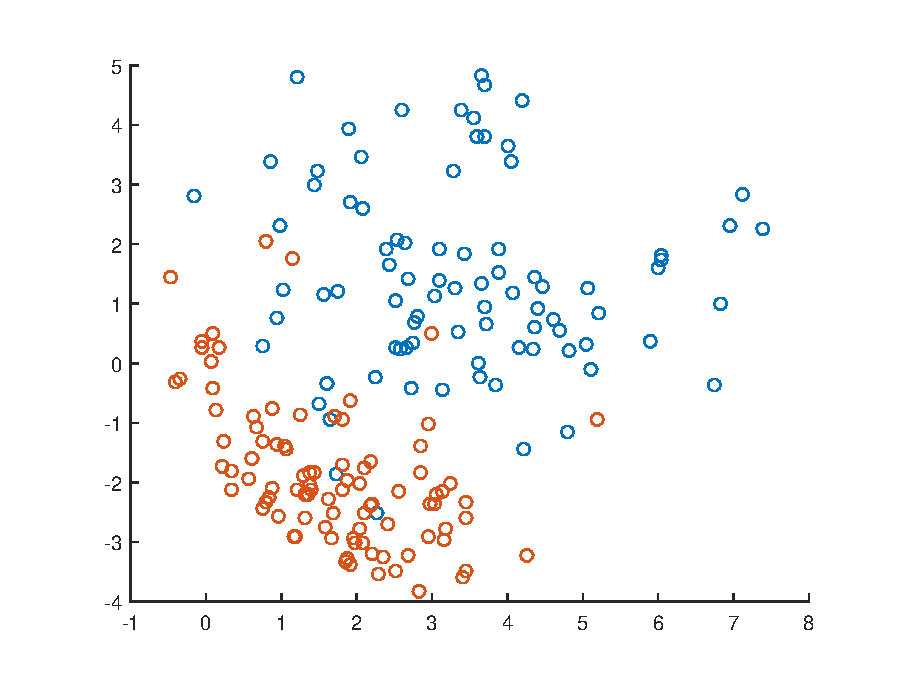
\includegraphics[scale=0.5]{figs/threeseightsKPCA.eps}         \caption{KPCA}
    \end{subfigure}
\quad \quad \quad \quad \quad \quad \quad 
    \begin{subfigure}[b]{0.3\textwidth}
\includegraphics[scale=0.5]{figs/thveireg.eps}         \caption{CKFD:Regular}
    \end{subfigure}
    \end{center}
    \caption{Distribution of digits 3 and 8.}     \label{fig:distances}
\end{figure}
\begin{table}[h]
\centering
\caption{Classification results for the methods on the MNIST handwritten digits.}
\label{my-label}
\begin{tabular}{|l|l|l|l|l|l|}
\hline
Method    & Classification Rate & (Training + Decision) Time & Kernel   & Parameter     & Fusion Coefficient \\ \hline
PCA+NN    & 89.5                & 0.27029s                   & -        & -             & -                  \\ \hline
PCA+MD    & 79.5                & 0.27029s                   & -        & -             & -                  \\ \hline
KPCA+NN   & 87.9                & 1.9044s                    & Gaussian & $ \sigma =5 $ & -                  \\ \hline
KPCA+MD   & 82.5                & 1.9044s                    & Gaussian & $ \sigma =5 $ & -                  \\ \hline
CKFD + NN & 93.2                & 2.4729s                    & Gaussian & $ \sigma =5 $ & $ \theta= 0.8 $    \\ \hline
CKFD + MD & 92.6                & 2.4729                     & Gaussian & $ \sigma =5 $ & $ \theta= 0.8 $    \\ \hline
\end{tabular}
\end{table}



\begin{table}[h]
\centering
\caption{Classification results for the methods on the Olivetti faces.}
\label{my-label}
\begin{tabular}{|l|l|l|l|l|l|}
\hline
Method    & Classification Rate & (Training + Decision) Time & Kernel   & Parameter      & Fusion Coefficient \\ \hline
PCA+NN    & 93.7500             & 0.29125s                   & -        & -              & -                  \\ \hline
PCA+MD    & 86                  & 0.29125s                   & -        & -              & -                  \\ \hline
KPCA+NN   & 93.5000             & 0.76282s                   & Gaussian & $ \sigma =40 $ & -                  \\ \hline
KPCA+MD   & 86                  & 0.76282s                   & Gaussian & $ \sigma =40 $ & -                  \\ \hline
CKFD + NN & 94                  & 0.82828s                   & Gaussian & $ \sigma =35 $ & $ \theta= 0.75 $   \\ \hline
CKFD + MD & 88                  & 0.82828s                   & Gaussian & $ \sigma =35 $ & $ \theta= 0.75 $   \\ \hline
\end{tabular}
\end{table}



\begin{multicols}{2}
\section{Instructions}
The directory contains a folder with scripts and a folder with the figures. The experiments run in two stages. 
Prepare the data. This can be done by either running 
$Olivetti.m$ or $prepMNIST.m$. This will set up the required data structures for the chosen dataset.
After that just run $crossv.m$. This script has 3 options. By commenting/uncommenting the corresponding line, the feature extraction/classification method can be picked. The 3 options are the ones that have been reported in the results, namely, CKFD+NN/MD, KPCA+NN/MD, PCA+NN/MD.



 \begin{thebibliography}{9}
 \bibitem{yang05}
 Yang, Jian, et al. "KPCA plus LDA: a complete kernel Fisher discriminant framework for feature extraction and recognition." Pattern Analysis and Machine Intelligence, IEEE Transactions on 27.2 (2005): 230-244.

\bibitem{schol98}
Schölkopf, Bernhard, Alexander Smola, and Klaus-Robert Müller. "Nonlinear component analysis as a kernel eigenvalue problem." Neural computation 10.5 (1998): 1299-1319. 
 
\bibitem{schol99}
Scholkopft, Bernhard, and Klaus-Robert Mullert. "Fisher discriminant analysis with kernels." Neural networks for signal processing IX 1 (1999): 1. 

\bibitem{hof06}
Hofmann, Thomas, Bernhard Schölkopf, and Alexander J. Smola. "A review of kernel methods in machine learning." Mac-Planck-Institute Technical Report 156 (2006). 

\bibitem{smola06}
Smola, Alex J., and Bernhard Schölkopf. "A tutorial on support vector regression." Statistics and computing 14.3 (2004): 199-222. 

\bibitem{murph12}
Murphy, Kevin P. Machine learning: a probabilistic perspective. MIT press, 2012.
  
 
 \end{thebibliography}
 

\end{multicols}
\end{document}